\documentclass[aspectratio=169]{beamer}

% because we need to claim weird things
\newtheorem{claim}{Claim}
\newtheorem{defn}{Definition}
%\newtheorem{lemma}{Lemma}
\newtheorem{thm}{Theorem}
\newtheorem{vita}{Vit\ae}
\newtheorem{qotd}{Quote of the Day}

\usepackage{algorithm}
\usepackage{algpseudocode}
\usepackage{listings}
\usepackage{color}
\usepackage{graphics}
\usepackage{ulem}
\bibliographystyle{unsrt}

% background image
\usebackgroundtemplate%
{%
    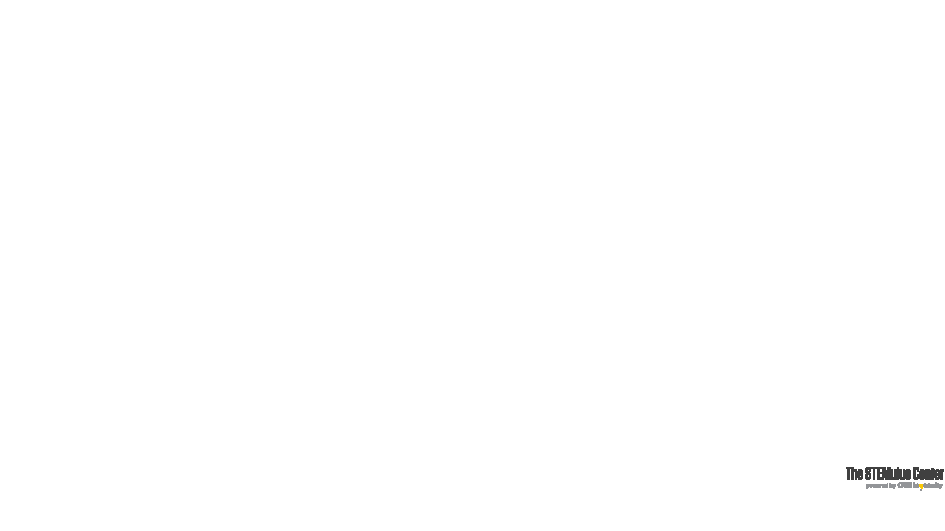
\includegraphics[width=\paperwidth,height=\paperheight]{../artifacts/stemulus.pdf}%
}
\setbeamertemplate{caption}[numbered]
\lstset{%
	breaklines=true,
	captionpos=b,
	frame=single,
	keepspaces=true,
	showstringspaces=false
}

% page numbers
\addtobeamertemplate{navigation symbols}{}{%
    \usebeamerfont{footline}%
    \usebeamercolor[fg]{footline}%
    \hspace{1em}%
    \insertframenumber/\inserttotalframenumber
}

% presentation header
\usetheme{Warsaw}
\title{Secure Development in an Insecure World}
\author{Dylan Lane McDonald}
\institute{CNM STEMulus Center\\Web Development with PHP}
\date{\today}

\begin{document}
\lstset{language=Java}
\begin{frame}
\titlepage
\end{frame}

\begin{frame}
\frametitle{Outline}
\tableofcontents
\end{frame}

\section{Introduction to Security}
\subsection{Security Triad}
\begin{frame}
\frametitle{What is Security?}
What is security?
\pause
\begin{enumerate}
	\item \textbf{Confidentiality}: the prevention of disclosure of information to unauthorized parties (known to laymen as ``privacy'')
	\item \textbf{Integrity}: the guarantee that the information has not be altered, delayed, or otherwise had its consistency compromised
	\item \textbf{Availability}: the state of having the information accessible once applicable security protocols and credentials have been provided
\end{enumerate}
A secure system is one that consists of all three of these properties. These seemingly conflicting objectives are depicted in Figure \ref{fig:cia}.

\mbox{}\\
Many lay people confuse ``security'' for solely the ``confidentiality'' aspect of it. As a result, many people overfocus on confidentiality and neglect integrity and availability.
\end{frame}

\begin{frame}
\frametitle{Security Triad}
\begin{figure}
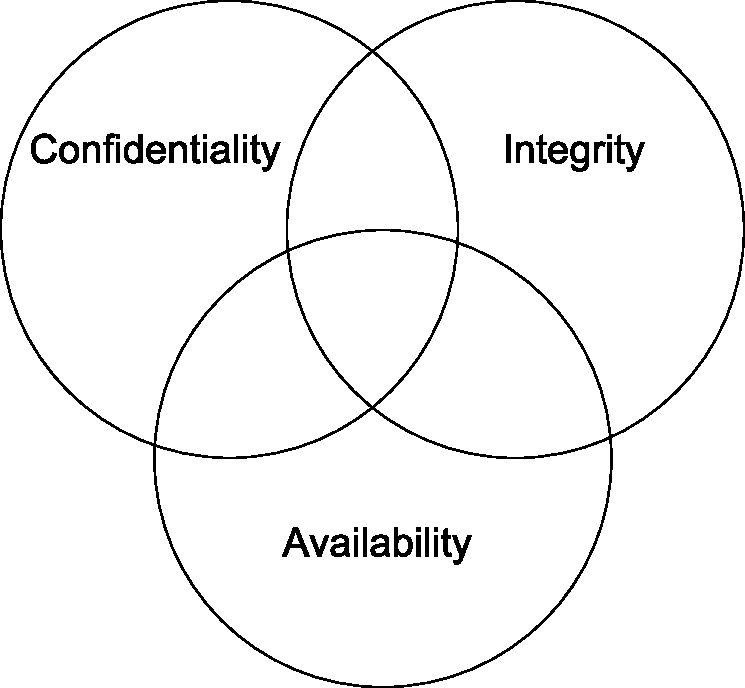
\includegraphics[scale=0.45]{../artifacts/cia.pdf}
\caption{Security Triad}
\label{fig:cia}
\end{figure}
\end{frame}

\subsection{Onion Model}
\begin{frame}
\frametitle{Onion Model}
In order to accomplish all three objectives in Figure \ref{fig:cia}, a multi-faceted solution is necessary.
\pause
\begin{defn}
The \textbf{onion model} is a common model illustrating the many ``layers'' of information security. The model, depicted in Figure \ref{fig:onion}, represents how the data can be protected by multiple strategies as it exists and interacts with a system.
\end{defn}

\pause
\mbox{}\\
The onion model has many roles played by many players, both in terms of system roles and physical (human) roles.
\end{frame}

\begin{frame}
\frametitle{Onion Model}
\begin{figure}
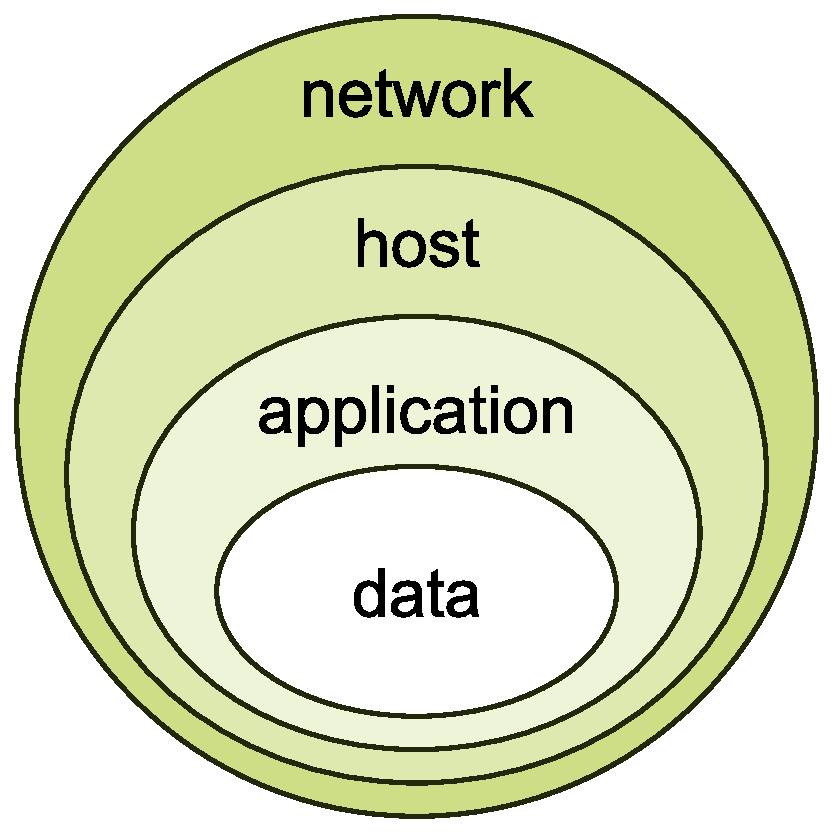
\includegraphics[scale=0.4]{../artifacts/onion.pdf}
\caption{Onion Model}
\label{fig:onion}
\end{figure}
\end{frame}

\begin{frame}
\frametitle{System Roles}
Some of the system roles in the onion model are:
\begin{itemize}
	\item \textbf{Firewall/Router}: prevents malicious traffic from ever contacting the application
	\item \textbf{Limitation of Access}: the less door one opens to the data, the less the chance the data will be compromised
	\item \textbf{Encryption}: scrambling data while transmitted or in storage to prevent attackers from reading data
	\item \textbf{Input Sanitization}: filtering inputs before they hit the application to minimize the chance of compromising the data's integrity
\end{itemize}
As a web developer, your most powerful and most used role in the onion model is$\dots$\pause\textbf{input sanitization}!
\end{frame}

\begin{frame}
\frametitle{Human Roles}
Humans are inevitably involved in the operation and development of any system. The major roles are:
\begin{itemize}
	\item \textbf{Systems Administrator}: responsible for setting up servers and routers and keeping internal data accessible only via secure methods
	\item \textbf{Software Architect}: responsible for deciding on how different methods will be implemented; often, these will have large security implications
	\item \textbf{Software Developer}: responsible for using good coding practices and programmatically preventing malicious users from succeeding
\end{itemize}
Working as a cohesive team, these three roles can create a united front against attacks and create secure software.
\end{frame}

\section{Cryptography}
\subsection{Meet the Players}
\begin{frame}
\frametitle{Meet the Players}
Security scenarios are almost always illustrated with the following players:
\begin{itemize}
	\item \textbf{Alice}, \textbf{Bob}, \& \textbf{Charlie}: ordinary end users who use the system
	\item \textbf{Eve}: an \emph{eavesdropper} listening to Alice \& Bob
	\item \textbf{Mallory}: a \emph{malicious} user who compromises Alice or Bob
\end{itemize}

There are more players on stage, but these are by far the most common.
\pause
\begin{vita}
\textbf{Ron Rivest}, \textbf{Adi Shamir} and \textbf{Leonard Adleman} developed the RSA encryption algorithm, which is the basis of encryption algorithms such as SSL, PGP, and SSH.
\end{vita}
\end{frame}

\subsection{Hashes}
\begin{frame}
\frametitle{Hashes}
A hash is the industry standard way for storing passwords.
\begin{defn}
A \textbf{hash} is a mathematical function $f: \mathcal{S} \rightarrow \mathbb{N}$ such that $H(x_1) \ne H(x_2)$ for all $x_1 \in \mathcal{S}$ and $x_2 \in \mathcal{S}$ and that $H^{-1}(x_1) = \emptyset$.
\end{defn}
Notice the definition of a hash guarantees two important properties:
\begin{enumerate}
	\item \textbf{Unique}: No two inputs will produce the same output
	\item \textbf{Singular}: Given an output $h$, there is no way to determine which input produced $h$
\end{enumerate}
These two reasons make hashes the ideal choice for storing passwords. Passwords are never stored in a database. Instead, given a password $p, H(p)$ is stored.
\end{frame}

\begin{frame}
\frametitle{Hash Algorithms}
There are two hash algorithms in use today: MD5 and SHA-2:
\begin{enumerate}
	\item \textbf{MD5}: A fast, efficient, \emph{insecure} hash algorithm. A collision (where $MD5(x_1) = MD5(x_2))$ has been found. MD5 is still present in legacy code and used as a signature where the security of the data is unimportant.
	\item \textbf{SHA-2}: A slower, fully secure hash algorithm. SHA-512\footnote{SHA-2 with a 512 bit output} is considered secure for storing and protecting sensitive information such as passwords and private keys.
\end{enumerate}

\mbox{}\\
Avoid using MD5 where possible. The US government now requires all software discontinue using MD5 and use SHA-2 instead.
\end{frame}

\begin{frame}
\frametitle{Birthday Attack: Setup}
Take a room with $n$ people in it. What is the probability that two people will be born on the same day?
\[P_d(n) = 1 - \left(\frac {364}{365}\right)^n\]
And what is the probability two people have the same birthday?
\[P_a(n) =  1 - \frac {365!} {(365 - n)! \cdot 365^n}\]
Intuitively, both $P_a(n)$ and $P_d(n)$ are quite small. However, if $n = 30$, $P_a(n) \approx 70.63\%$ and $P_d(n) \approx 7.901\%$.
\end{frame}

\begin{frame}
\frametitle{Birthday Attack: Impact}
Given a function $H(x)$, find two inputs $x_1$ and $x_2$ such that $H(x_1) = H(x_2)$ (i.e., a collision). How much work needs to be done to find a collision? Matching the terms to the previous slide:
\begin{enumerate}
	\item \textbf{Birthday Problem}: hash function
	\item \textbf{People}: inputs to the hash function
	\item \textbf{People's Birthdays}: outputs to the hash function
\end{enumerate}
The impact of the birthday attack is an exact measure of how difficult it is to find a random collision for a hash function. This is why hashes are \textbf{birthday bound}. For instance, a 128 bit hash is birthday bound at $2.2 \times 10^{19}$ since, on average, it will take $2.2 \times 10^{19}$ attempts to find a collision.
\end{frame}

\subsection{Encryption}
\begin{frame}
\frametitle{Symmetric Encryption}
\textbf{Problem}: Alice wants to send a message to Bob securely.

\mbox{}\\
\textbf{Solution}: Alice encrypts her message with a \textbf{private key}, $k$. She then uses $k$ to transform the message to something Eve cannot read without previous knowledge of $k$. Bob receives the message and uses $k$ to transform the message back to its original state.

\begin{defn}
The scenario just outlined is known as \textbf{symmetric encryption}. Symmetric encryption requires that Alice and Bob have the same secret information in common, the private key $k$.
\end{defn}
Any symmetric encryption scenario is just as secure as the storage \& exchange of $k$.
\end{frame}

\begin{frame}
\frametitle{Asymmetric Encryption}
\textbf{Problem}: Alice wants to send a message to Bob securely.

\mbox{}\\
\textbf{Solution}: Alice sends her public key $P_a$ to Bob. Bob replies with his public key $P_b$. Alice then encrypts the message using her private key, $K_a$ and $P_b$. Bob receives the message and decrypts the message using his private key, $K_b$ and $P_a$. 

\begin{defn}
The scenario just outlined is known as \textbf{asymmetric encryption}. Asymmetric encryption is considered more secure because the public keys are by definition public and don't need to be protected. The private keys are assigned per user and one user doesn't want/need to know the other user's private key.
\end{defn}
\end{frame}

\begin{frame}
\frametitle{Common Encryption Algorithms}
\begin{table}
\begin{tabular}{|l|l|p{4cm}|}
\hline
\textbf{Algorithm} & \textbf{Type} & \textbf{Comment}\\
\hline
3DES & Symmetrical & Used internally in credit card systems\\
\hline
AES & Symmetrical & Current standard for symmetrical algorithms\\
\hline
Diffie-Hellman & Asymmetrical & Used in secure key exchange schemes\\
\hline
RSA & Asymmetrical & Underlying algorithm for PGP, SSH, \& SSL\\
\hline
\end{tabular}
\caption{Common Encryption Algorithms}
\label{tbl:algorithms}
\end{table}
\end{frame}

\section{Attacks}
\subsection{SQL Injection}
\begin{frame}
\frametitle{SQL Injection}
\begin{figure}
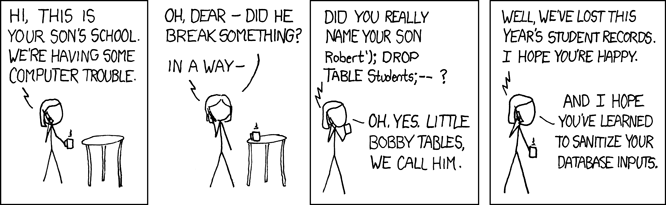
\includegraphics[scale=0.6]{../artifacts/bobby-tables.png}
\caption{SQL Injection Attack \cite{xkcd}}
\label{fig:bobbytables}
\end{figure}
\end{frame}

\begin{frame}
\frametitle{SQL Injection}
What the comic in Figure \ref{fig:bobbytables} is referencing is when HTML form fields directly reference/affect a database table. When these inputs are not sanitized, an attacker can use carefully crafted inputs to make the system perform actions that are not expected, usually by elevating an unauthorized user to a higher status.

\mbox{}\\
The key solution to this problem is \textbf{input sanitization} and using prepared statements. This preprocessing step reduces the vulnerability of sites and prevents the malicious inputs from executing on the SQL server.
\end{frame}

\subsection{Cross Site Scripting (XSS)}
\begin{frame}
\frametitle{Cross Site Scripting (XSS)}
\textbf{Cross site scripting (XSS)} allows an attacker to inject arbitrary code into a web site. For instance, say Alice visits Bob's site, which has a login system and a search engine. Alice searches for \textit{foo} while logged into Bob's site. Bob's site typically displays something about the query for \textit{foo}. Mallory knows this and sends Alice an Email enticing her to search for \textit{foo} again. Mallory's Email exploits a weakness in Bob's input sanitizations and hijacks Alice's session and allows Mallory's full control over Alice's account.

\mbox{}\\
This is known as a \textbf{non-persistent} attack and is by far the most common cross site scripting attack.
\end{frame}

\begin{frame}
\frametitle{Cross Site Scripting}
Extending the example from the previous slide, suppose Mallory posts a link to Bob's site on a social media site or forum. The link contains hidden code that allows Mallory to take control of any unsuspecting visitors who click the link. This is a \textbf{persistent} attack.

\pause
\mbox{}\\
The solution to both these attacks is simple: \textbf{input sanitization}. By not trusting user inputs and stripping potential attack vectors (e.g., HTML tags), Bob's site is no longer vulnerable to cross site scripting attacks.
\end{frame}

\subsection{Cross Site Request Forgery (CSRF)}
\begin{frame}
\frametitle{Cross Site Request Forgery (CSRF)}
\textbf{Cross Site Request Forgery (CSRF)}, like XSS, allows an attacker to exploit Alice's open session. In CSRF, the attacker uses a link to one site to exploit Alice's session on another site. For instance, suppose Alice has an active session at Bob Bank. Mallory sends an Email (or posts a message on social media) that contains \texttt{POST} variables that will manipulate Alice's session at Bob Bank, such as changing her password or emptying her balance.

\pause
\mbox{}\\
The solution to CSRF is to randomly generate a challenge/response with every \texttt{POST} operation. Mallory, at best, can see the contents of cookies, but not the contents of the session. By verifying a challenge and response every time, Bob Bank ensures that the request came from Alice.
\end{frame}

\section{Safe Coding Principles}
\begin{frame}
\frametitle{Safe Coding Principles}
What can a developer do to prevent attacks in the first place?
\pause
\textbf{\emph{INPUT SANITIZATION}}

\pause
\mbox{}\\
In addition, whenever a user account is created (an SQL user, an account an end-user signs up for, etc.), give that user minimal control over the system. This is known as the \textbf{Principle of Least Privilege}. \cite{owasp} For instance, it is common practice to have a ``super user''\footnote{Often referred to as ``root''} that has full control of a database and an ``application user'' that is limited to \texttt{DELETE}, \texttt{INSERT}, \texttt{SELECT}, and \texttt{UPDATE}. Any schema changes, imports, or other ``powerful'' changes are done by the root user. The web application is only granted access to the more limited application user.
\end{frame}

\begin{frame}
\frametitle{Coding with a Safe Attitude}
Following a few simple rules will facilitate a secure mindset:
\begin{itemize}
	\item \textbf{Trust Nothing}: Always suppose the server, mySQL instance, etc. are compromised. Write your code as if nothing but malicious users use your program.
	\item \textbf{Keep Code Simple}: Simpler code has less of an opportunity for bugs that will potentially open security vulnerabilities.
	\item \textbf{Principle of Least Privilege}: Carefully consider to what extent any user accounts have in your system and limit their access to the absolute minimum.
	\item \textbf{Input Sanitization}: All inputs sent to a system are unsafe. This is the most effective technique in secure coding.
\end{itemize}
\end{frame}

\begin{frame}
\frametitle{Works Cited}
\bibliography{security}
\end{frame}
\end{document}